\setchapterstyle{lines}
\labpage{appendix}
%\blinddocument

\chapter{在$x=0$处展开的泰勒级数多项式与被展开的函数图像比对}
\begin{thm}
    $$e^x=1+x+\dfrac{x^2}{2!}+\dfrac{x^3}{3!}+\cdots+\dfrac{x^n}{n!}+\cdots$$
\end{thm}
\begin{figure}[h]
	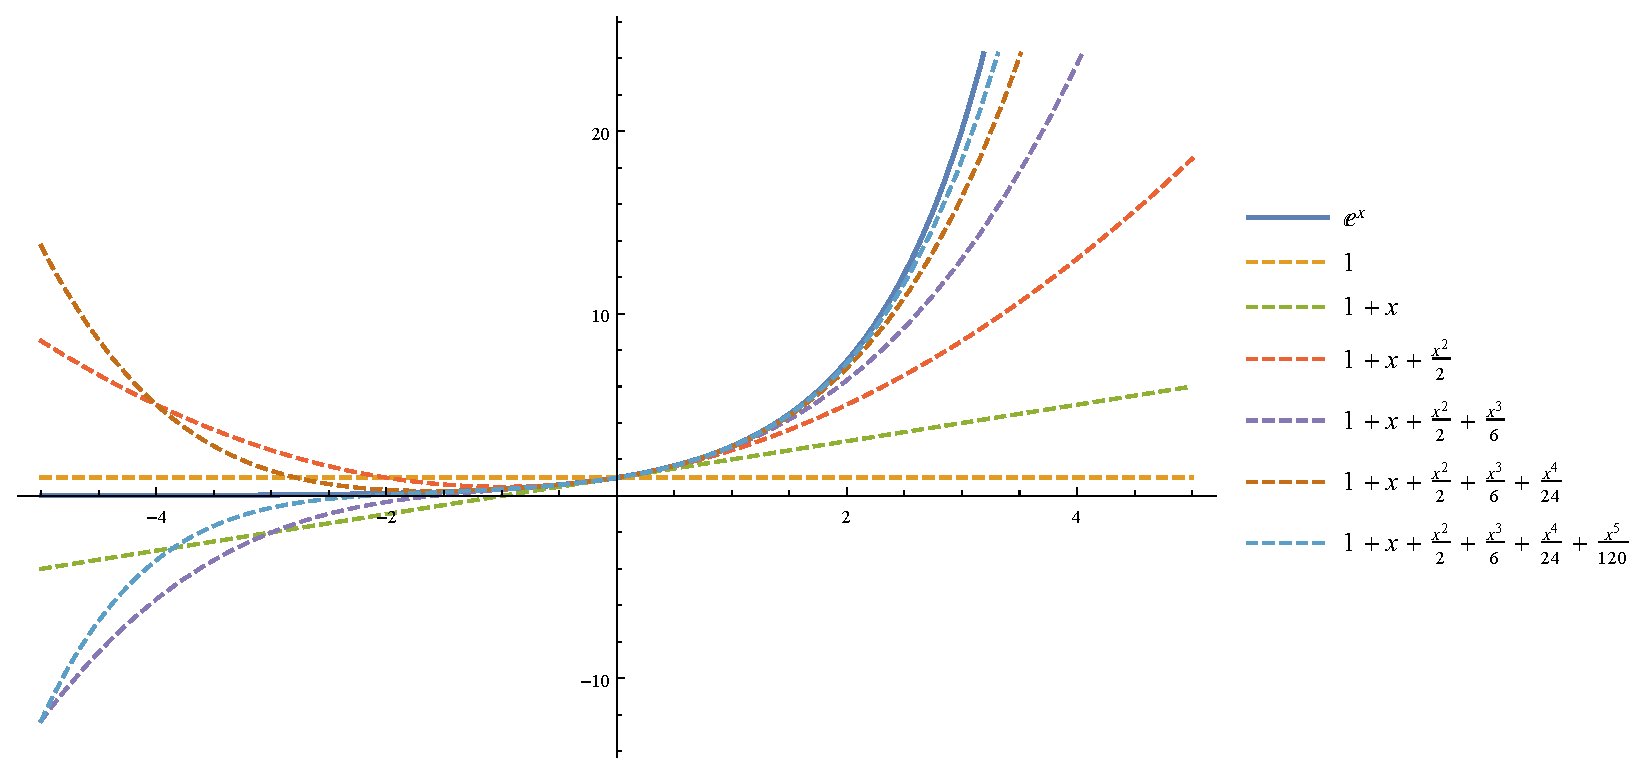
\includegraphics[width=\textwidth]{Figure-13-e^x.eps}
	\caption[figex]{$f(x)=e^x$在$x=0$处展开后的截断多项式的图像和原函数图像。}
\end{figure}\par
\begin{thm}
    $$\ln(1+x)=x-\dfrac{x^2}{2!}+\dfrac{x^3}{3!}-\cdots+(-1)^{n+1}\dfrac{x^{n}}{n!}+\cdots$$
\end{thm}
\begin{figure}[h]
	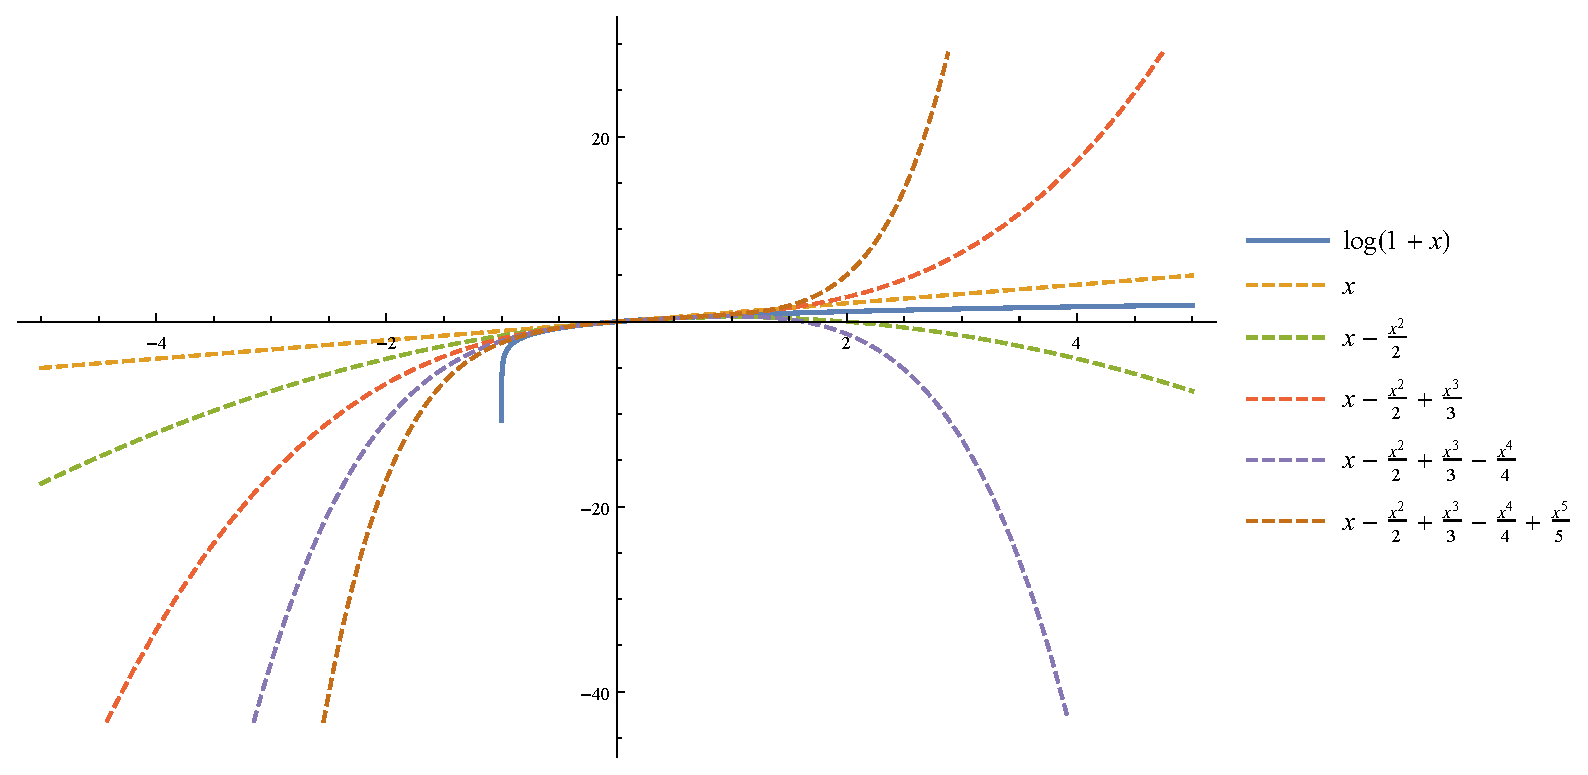
\includegraphics[width=\textwidth]{Figure-14-lnx.eps}
	\caption[figln]{$f(x)=\ln(1+x)$在$x=0$处展开后的截断多项式的图像和原函数图像。}
\end{figure}\par
\begin{thm}
    $$\sin x=x-\dfrac{x^3}{3!}+\dfrac{x^5}{5!}-\cdots+(-1)^{n}\dfrac{x^{2n+1}}{(2n+1)!}+\cdots$$
\end{thm}
\begin{figure}[h]
	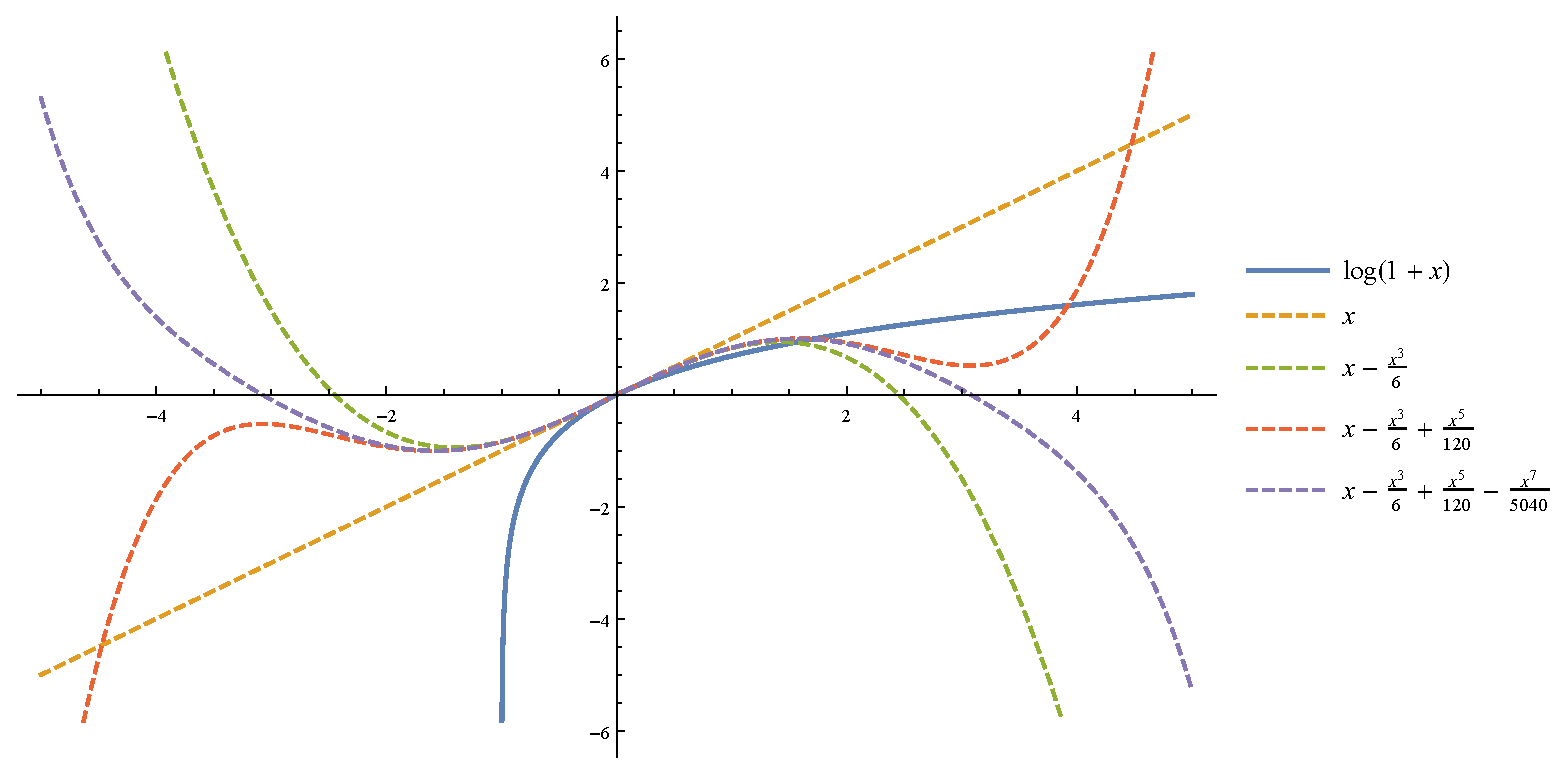
\includegraphics[width=\textwidth]{Figure-15-sinx.eps}
	\caption[figln]{$f(x)=\sin x$在$x=0$处展开后的截断多项式的图像和原函数图像。}
\end{figure}\par
\begin{thm}
    $$\cos x=1-\dfrac{x^2}{2!}+\dfrac{x^4}{4!}-\dfrac{x^6}{6!}+\cdots+(-1)^n\dfrac{x^{2n}}{(2n)!}+\cdots$$
\end{thm}
\begin{figure}[h]
	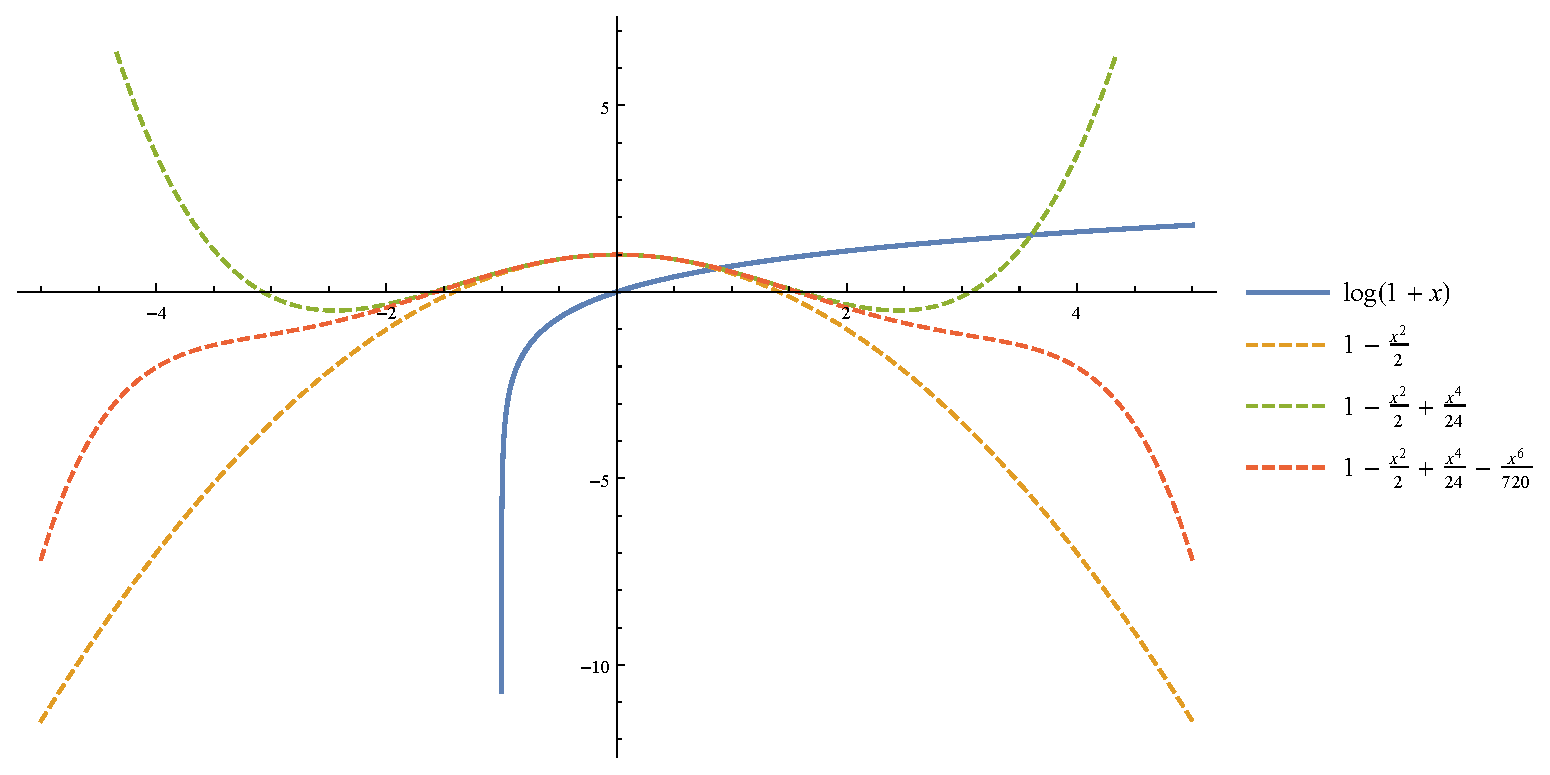
\includegraphics[width=\textwidth]{Figure-16-cosx.eps}
	\caption[figln]{$f(x)=\cos x$在$x=0$处展开后的截断多项式的图像和原函数图像。}
\end{figure}